\section{Overview of control}
\label{sc:control}
This is an overview of the information flow for control in regard to the rest of the system containing, sensors, \ac{LLI} and \ac{HLI}.

\begin{figure}[htbp]
	\centering
	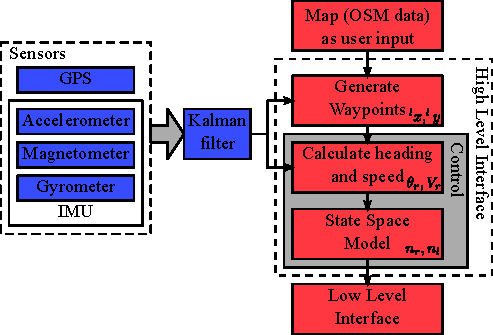
\includegraphics[width=\textwidth]{img/vessel-block-overview}
	\caption{Overview of control information flow in regard to the subsystems. The blue part indicates information that is not fetched directly to the control part, it is electrically connected to the \ac{LLI} whilst being forwarded to the \ac{HLI}.}
	\label{fig:vessel-block-overview}
\end{figure}

\todo{Illustrate on figure~\vref{fig:vessel-block-overview} where RF comms is or maybe that should be on the block overvieww diagram without regard to contorl abstraction}

\section{Designing the State Space Model}

\subsection{Choosing the right states}

\todo{Why we chose a lot of states in the beginning, and then were left with just a few, talk about that}

\subsection{Linearizing the outputs}

Using Newton's second law of motion for forward  and rotational movement (F = m * A; T = I * W'), we can easily see that the inputs to our system will be F and T representing the forward force and the torque produced by the motors. It is worth mentioning that, since there are two propellers rotating in opposite directions, a torque that would induce a rotation around Z axis passing through the boat's center of mass only if the two propellers are rotating at different speeds.

These two rotational speeds N1 and N2 were initially included in the state space model as inputs to the system, as they could be controlled directly via a PWM pulse. This though proved to complicate matters because the relationship between the speeds of the propellers N1 and N2 and the force F and torque T generating accelerations is not a linear one. Because of this, our system would not be linear and would be beyond the scope of this project. 

\todo{insert formulas for this transformation here}

In order to prevent this from happening, the state space model was updated to only calculate the force T and torque T necessary for driving and turning the ship, and this would keep our system linear. in order to transform from [T, F] to [N1, N2], another module was introduced in the system which would implement this non-linear function. 

This is a better solution anyway because if the state space model only outputs T and F, then it could be used for some other ship configurations, without modifications to the model, only to the module that translates the force and torque to N1 and N2. This, for example, can allow us to change the size of the propellers or their positions.

\subsection{Linearizing the drag forces}

The drag forces acting on the bow of the ship while it's moving through the water are influenced by the area of the hull that is below water depth in the direction of movement, the density of the water, a constant C (which also includes a form factor, which for the moment, is considered to be a box), and the square of the ship's speed $ v $

\[ D(v) = \frac{C_{D}\cdot\rho_{water}\cdot A_{hull}\cdot v^{2}}{2} \]

Where $D(v)$ is the drag force dependent on the forward speed, $C_{D}$ is the drag coefficient, $\rho_{water}$ is the density of the water, $A_{hull}$ is the frontal area of the hull. 

The drag torque that is produced by the drag force acting on the hull of the ship, as the ship rotates through the water is dependent on the square of the angular velocity $ \omega $.

\[ \tau(\omega) = \frac{C_{D} \cdot \rho_{water} \cdot d \cdot (r_{f}^{4} + r_{b}^{4}) \cdot \omega^{2}}{8} \]

Where $ \tau(\omega) $ is the torque generated by the angular speed $ \omega $, $ d  $ is the depth of the ship that is submerged in water, $ r_{f} and r_{b} $ are the radii of the ship from the center of mass towards the front and back end, respectively.

These forces are obviously non-linear and thus cannot be integrated into the linear Kalman filter or State Space Model. Because we will usually use a constant speed it is feasible to linearize these forces for that value and not have big errors. The angular drag torque can also be linearized around a mean turning speed because the radii of the corners of the paths (where we will turn) are also constant.

\todo{Formulas and calculations for linearizing}


